% !TEX program = lualatex
% !TEX recipe = latexmk (lualatex)
\pdfvariable minorversion = 4
\pdfvariable objcompresslevel = 0
\documentclass{sice-si}

\def\LuaLaTeX{Lua\LaTeX}
\def\upLaTeX{up\LaTeX}
\def\pTeX{p\TeX}
\def\SICEcls{sice.cls}

\newcommand{\TeXEngine}{unknown}
\ifluatex
    \renewcommand{\TeXEngine}{\LuaLaTeX}
\else
    \ifuptex
        \renewcommand{\TeXEngine}{\upLaTeX}
    \fi
\fi

\usepackage{cite}

% タイトルと著者名
\title{シミュレーション環境における生成的群衆行動のための蒸留ビヘイビアツリーに基づくモデリング} % 和文タイトル
\name{○NGUYEN TRI TUNG NGUYEN，細田侑也，李俊浩（立命館大学）} % 著者名
\etitle{Distilled Behavior Tree-Based Modeling For Generative Crowd Behavior in Simulation Environment.} % 英文タイトル
\ename{○Tri Tung Nguyen NGUYEN, Yuya HOSODA, and Joo-Ho LEE (Ritsumeikan University)}	%著者名（英）

\begin{document}
% アブストラクト
\abst{
    Although modern generative crowd architectures offer broad and high-quality behavioral coverage, their substantial runtime computational overhead impedes closed-loop deployment. To address this, we propose a novel behavior-tree-based generative framework that distills neural policies into explainable, deterministic structures suitable for closed-loop robotic simulations.
}

% タイトルの出力
\maketitle

% 本文
\section{緒言}
都市環境で稼働する自動運転車やサービスロボットの評価には，現実的な群衆シミュレーションが不可欠である．古典的な歩行者モデルであるSocial Force Model（SFM）\cite{helbing1995social}やOptimal Reciprocal Collision Avoidance（ORCA）\cite{vandenberg2011reciprocal}は，計算効率に優れる．しかし，明示的なヒューリスティクスに基づくため，実際の群衆が示す行動の多様性や多峰性を捉えにくい．
\begin{figure*}[t]
    % First photo
    \centering
    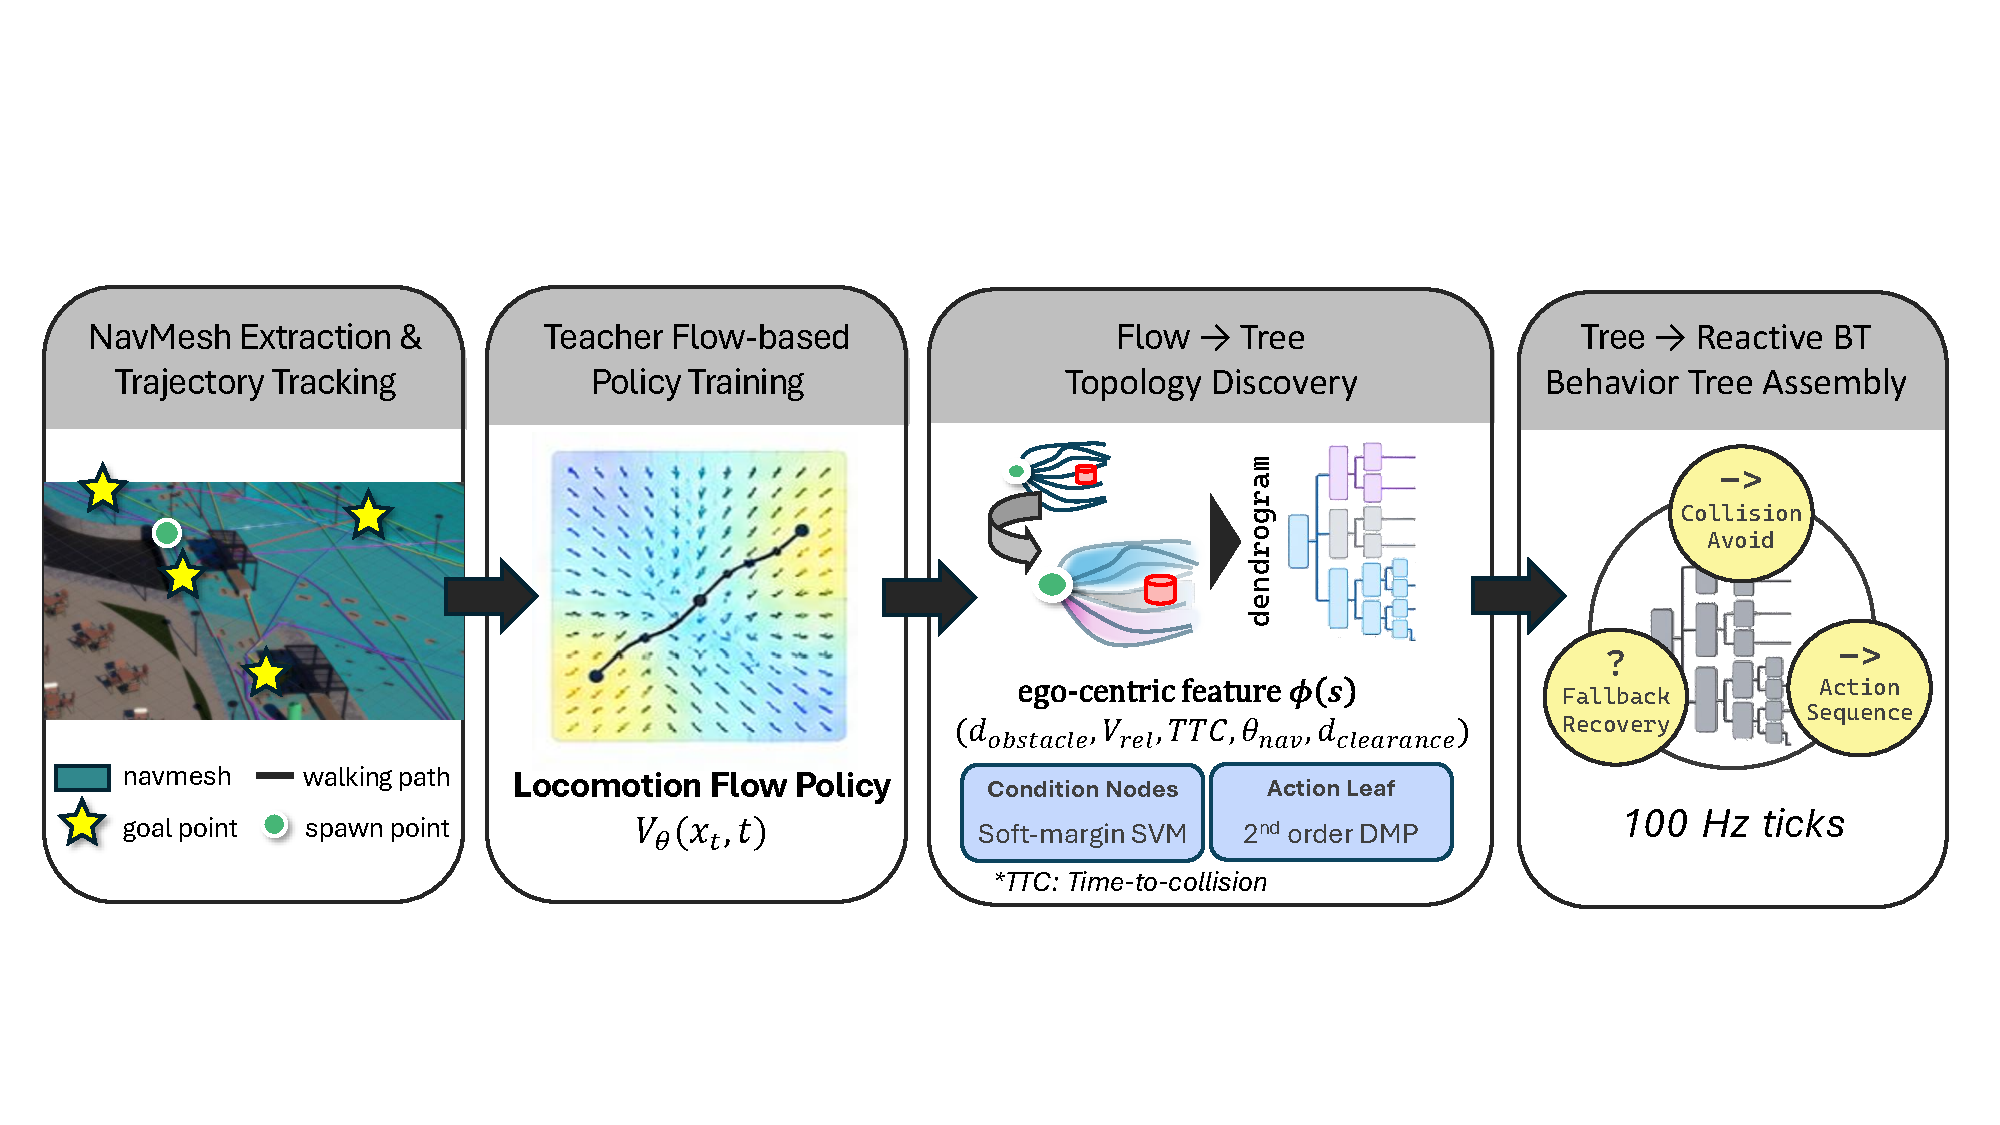
\includegraphics[width=0.82\textwidth,trim={0.6cm 3.5cm 0.8cm 3.5cm},clip]{figures/overview.pdf}
    \vspace{-1mm}
    \caption{
         Overview of the proposed Flow2BT framework. The generative flow matching model is used as a teacher to distill continuous multimodal pedestrian behaviors into a reactive, interpretable Behavior Tree (BT) with closed-form Dynamical Movement Primitive (DMP) leaves.
    }
    \label{fig:overview}
    \vspace{-2mm}
\end{figure*}

近年では，CrowdES~\cite{bae2025crowdes}のように，フローマッチング（Flow Matching）\cite{lipman2023flow}により実測データから連続的な速度場を学習する深層生成モデルが提案されている．しかし，これらを閉ループシミュレーションに組み込むと，二つの課題が生じる．第一に，モードは開ループの時間チャンク（$T_f = 2\,\text{s}$）ごとに一度しか予測されないため，その間エージェントは周囲の変化に反応できない（意思決定遅延）．第二に，ニューラルデコーダは記号的な論理を持たないため，道を譲る，回避する，停止するといった判断の根拠を検証できない（ブラックボックス性）．

本稿では，連続的な生成群衆方策を解釈可能なビヘイビアツリー（Behavior Tree; BT）\cite{colledanchise2018behavior}へ蒸留するフレームワーク\textbf{Flow2BT}を提案する．Flow2BTは，木とフローの双対性\cite{ramachandran2026trees}に基づき，生成フローモデルを教師としてナビゲーションメッシュ（NavMesh）座標系で分岐構造を抽出する．各分岐は，線形の条件ノードと2次の動的運動プリミティブ（Dynamical Movement Primitives; DMP）\cite{chatzilygeroudis2021behavior}に変換される．得られたBTは$100\,\text{Hz}$でtickされ，Fallbackノードによるプリエンプションを伴う$10\,\text{ms}$周期の制御更新を実現する．本研究の主な貢献は以下の3点である．(1) 連続的な群衆方策を，閉形式のDMPを葉に持つ解釈可能なBTへ蒸留できることを示し，$2000\,\text{ms}$の開ループチャンクに対して$100\,\text{Hz}$での反応的な評価を可能にする．(2) 正解軌道から導出したBTがCrowdESの巨視的な空間密度と人数分布を保持することを20回の対応のある試行により示し，フロー教師から蒸留した場合に残る現実性の差を定量化する．(3) 単峰的なアクションノードを閉形式のDMPとしてパラメータ化し，開ループチャンクによる遅延なしに滑らかな移動を実現する．

\section{関連研究}
\subsection{歩行者移動の生成モデル}
歩行者シミュレーションは，SFM\cite{helbing1995social}やORCA\cite{vandenberg2011reciprocal}などのルールベースモデルから，表現力の高いデータ駆動型の手法\cite{alahi2016social,lipman2023flow}へと発展してきた．CrowdES~\cite{bae2025crowdes}は，NavMeshのウェイポイントを条件とした連続的な群衆生成を実現している．しかし，既存の生成的シミュレータは開ループのチャンク処理（$T_f = 2\,\text{s}$，$5\,\text{fps}$）に依存しており，モード（$B=8$）をチャンクごとに一度しかサンプリングしない．密な群衆では，このホライズンに拘束されたエージェントが周囲の歩行者の動きに反応できず，硬直した軌道や停止によるデッドロックが生じる．

\subsection{ビヘイビアツリーとロボット制御}
BTは，Sequence（$\to$）ノードとFallback（$?$）ノードにより，モジュール性と反応性を備えたロボットの実行を実現し\cite{colledanchise2018behavior,iovino2022survey}，透明な検証とプリエンプションを可能にする．しかし，遺伝的プログラミングによるBTの合成\cite{iovino2022survey}では木の肥大化（bloat）が生じ，微分可能な緩和\cite{huang2025differentiable}では実運用時に大きな離散化ギャップが生じる．
軌道ベースのBTやDMP\cite{chatzilygeroudis2021behavior,ijspeert2013dynamical}は，連続的な実行と記号的な切り替えを橋渡しする．近年，RamachandranとSra\cite{ramachandran2026trees}は，連続的な速度場が逆時間方向において階層的なデンドログラムへ自然に粗視化されることを示した．Flow2BTはこの双対性に基づき，フロー方策を教師として用いることで，文法探索を必要とせずに解釈可能なBTの構造を導出する．

\section{提案手法}
\Fig{fig:overview}に示すように，Flow2BTは，高い表現力を持つ連続的な生成群衆方策を，解釈可能かつ反応的なBTへ体系的に蒸留する．処理は，相互に連携する以下の三つの段階から構成される．
\begin{enumerate}[label=\arabic*), labelsep=0.5em]
    \item \textbf{教師フロー方策の学習：}大域的なNavMesh追従と自己中心的なマルチエージェント文脈を条件として，連続的な移動ベクトル場を学習する．
    \item \textbf{フローからの木構造抽出：}連続的な軌道のアンサンブルをロールアウトし，逆時間の粗視化により階層的な決定デンドログラムを抽出する．
    \item \textbf{木構造からの反応的BTの構築：}最大マージンの条件ガードを導出し，アクションノードを2次のDMPとしてパラメータ化する．そのうえで，閉形式で行動を実行する$100\,\text{Hz}$の反応的BTを構築する．
\end{enumerate}

\subsection{教師フロー方策の学習}
\textbf{NavMeshによる誘導と幾何表現：}
各歩行者エージェント$i$の動的状態を$\mathbf{s}_i = [\mathbf{p}_i^\top, \mathbf{v}_i^\top]^\top \in \mathbb{R}^4$とする．ここで，$\mathbf{p}_i \in \mathbb{R}^2$は位置，$\mathbf{v}_i \in \mathbb{R}^2$は速度である．CrowdES~\cite{bae2025crowdes}に従い，歩行可能な領域を，Recastナビゲーションツールセット\cite{mononen2009recast}を用いて凸多角形からなるNavMeshへ離散化する．大域経路を繰り返し計算する代わりに，エージェントの生成時に一度だけ大域的な$A^*$探索を実行し，実行時にはエージェントの現在座標をキャッシュした折れ線へ射影する．これにより，局所的な先読みウェイポイント$\mathbf{c}_{i, \text{nav}} \in \mathbb{R}^2$（\Fig{fig:overview}左）を提供しつつ，経路探索のクエリ数を$600\times$以上削減する．

\textbf{自己中心的知覚特徴量：}
周囲の幾何的なアフォーダンスと歩行者間の動的な相互作用を捉えるため，各エージェントは\Fig{fig:overview}のセンサ構成に対応する自己中心的な特徴ベクトル$\phi(\mathbf{s}_i) \in \mathbb{R}^d$を構成する．
\begin{equation}
    \phi(\mathbf{s}_i) = \begin{bmatrix}
    d_{\text{obstacle}} \\
    \mathbf{v}_{\text{rel}} \\
    \text{TTC} \\
    \theta_{\text{nav}} \\
    d_{\text{clearance}}
    \end{bmatrix} = \begin{bmatrix}
    \|\mathbf{p}_{\text{obs}} - \mathbf{p}_i\| \\
    \mathbf{v}_j - \mathbf{v}_i \\
    \|\mathbf{p}_j - \mathbf{p}_i\| / (\|\mathbf{v}_j - \mathbf{v}_i\| + \epsilon) \\
    \angle(\mathbf{c}_{i, \text{nav}} - \mathbf{p}_i) - \angle(\mathbf{v}_i) \\
    \min(d_{\text{left}}, d_{\text{right}})
    \end{bmatrix}
\end{equation}
ここで，$d_{\text{obstacle}} \in \mathbb{R}$は最も近い静的境界までの距離（m），$j$は最も近い動的な歩行者のインデックスである．$\text{TTC}$は推定した衝突余裕時間（Time-to-Collision; s）であり，静止または同方向に移動する歩行者に対しては$\epsilon = 10^{-4}\,\text{m/s}$により安定化する．また，$\theta_{\text{nav}}$はNavMeshウェイポイントに対する進行方向の偏差（rad），$d_{\text{clearance}}$は横方向の通路境界までの距離（m）を表す．

\textbf{フローマッチングによる移動方策：}
マクロな教師モデルは，離散的なマルコフ状態遷移や確率的な拡散ステップではなく，連続速度場$v_\theta(\mathbf{x}_t, t, \mathbf{C}_s)$として定式化する．この速度場は，条件付きフローマッチング（Conditional Flow Matching; CFM）\cite{lipman2023flow}により学習する．$p_1$を，文脈$\mathbf{C}_s = [\phi(\mathbf{s}_i), \mathbf{c}_{i, \text{nav}} - \mathbf{p}_i]$を条件とする歩行者の歩行変位$\mathbf{x}_1 = \mathbf{v}_{\text{demo}} \in \mathbb{R}^2$（$\text{m/s}$）の経験的な目標分布とし，$p_0 = \mathcal{N}(0, \mathbf{I})$を標準ガウス事前分布とする．このとき，条件付き最適輸送（Optimal Transport; OT）確率パスを次式で定義する．
\begin{equation}
    \mathbf{x}_t = (1 - t)\mathbf{x}_0 + t \mathbf{x}_1, \quad \dot{\mathbf{x}}_t = \mathbf{x}_1 - \mathbf{x}_0, \quad t \in [0, 1]
\end{equation}
ニューラルベクトル場$v_\theta$は，隠れ層の次元が$[256, 512, 512, 256]$の4層MLPと，$128$次元の正弦波時間埋め込みによりパラメータ化する．条件ベクトル$\mathbf{C}_s$は，8フレーム（$1.6\,\text{s}$）の観測履歴に対し，CrowdESの文脈エンコーダ（潜在次元256，隠れ次元2048）により埋め込む．ネットワークは，ETHの標準学習データ分割を用い，AdamW（学習率$10^{-4}$）により次の平均二乗フロー回帰損失を最小化して学習する．
\begin{equation}
    \mathcal{L}_{\text{CFM}}(\theta) = \mathbb{E}_{t, \mathbf{x}_0, \mathbf{x}_1, \mathbf{C}_s} \left[ \left\| v_\theta(\mathbf{x}_t, t, \mathbf{C}_s) - (\mathbf{x}_1 - \mathbf{x}_0) \right\|_2^2 \right]
\end{equation}
得られる直線的なベクトル場は曲率に起因するアーティファクトを除去し，群衆における自然な譲歩や道を譲る動作を捉えた，高忠実度かつ多峰的な速度を生成する．

\subsection{フローからの木構造抽出}
\textbf{アンサンブル軌道のロールアウト：}
学習済みの連続フロー方策を生成的な教師として用い，多様な初期状態$\mathbf{s}_0 \sim \mathcal{S}_0$から$M$本の軌道をオフラインでロールアウトする．
\begin{equation}
    \Xi = \{\xi_k(\tau)\}_{k=1}^M, \quad \frac{d\xi_k}{d\tau} = v_\theta(\xi_k(\tau), \tau, \mathbf{C}_s^{(k)}), \quad \tau \in [0, T_f]
\end{equation}
ODEは，適応刻みのDormand-Prince法により，ホライズン$T_f = 2.0\,\text{s}$（$\Delta t = 0.2\,\text{s}$，将来10ステップ）にわたって積分する．多峰的な分岐を捉えるため，$S = 1,024$個の異なる文脈状態に対し，状態あたり$R = 16$本の確率的ロールアウトを生成する（$1024 \times 16$，計$M = 16,384$本）．

\textbf{逆時間フロー粗視化とデンドログラムの抽出：}
木とフローの双対性\cite{ramachandran2026trees}に従い，連続的な流線を時間の逆方向（$\tau = T_f - t$）にたどると，多峰分布が粗視化される．これにより，異なる軌道は次のペアワイズのスペクトル距離に基づき，自然に階層的なクラスタへまとめられる．
\begin{align}
    D(\xi_i, \xi_j) &= \int_0^{T_f} \|\xi_i(t) - \xi_j(t)\|_2^2 \, dt + \lambda_{\text{term}} \|\Delta \xi_{ij}(T_f)\|_2^2 \nonumber \\
    &\quad + \lambda_{\text{vel}} \int_0^{T_f} \|\dot{\xi}_i(t) - \dot{\xi}_j(t)\|_2^2 \, dt
\end{align}
ここで，$\Delta \xi_{ij}(T_f) \triangleq \xi_i(T_f) - \xi_j(T_f)$は終端における変位の差を表す．Wardの階層的クラスタリングにより，二分木のデンドログラム$\mathcal{T}_{\text{topo}}$を構築する（\Fig{fig:overview}中央）．分散が閾値$\epsilon_{\text{split}}$を超えるノード$k$を分岐ノードとして検出し，軌道を$B=8$個の単峰的な葉バンドル$\Xi_\ell$に分割する．

\subsection{木構造からの反応的BTの構築}
\textbf{ソフトマージンSVMによる条件ノードの導出：}
各分岐ノード$k \in \mathcal{T}_{\text{topo}}$において，子クラスタ$\Xi_{\text{left}}^{(k)}$と$\Xi_{\text{right}}^{(k)}$から二値ラベル$y \in \{+1, -1\}$を定める．遭遇の開始時点で収集した自己中心的な特徴量$\phi(\mathbf{s})$を用いて，ソフトマージンSVMを学習する（\Fig{fig:overview}右）．
\begin{align}
    \min_{\mathbf{w}_k, b_k, \boldsymbol{\xi}} \ & \frac{1}{2} \|\mathbf{w}_k\|_2^2 + C \sum_{m=1}^{M_k} \xi_m \\
    \text{s.t.} \ & y_m (\mathbf{w}_k^\top \phi(\mathbf{s}_{i, m}) + b_k) \ge 1 - \xi_m, \quad \xi_m \ge 0 \nonumber
\end{align}
実行時，条件述語は$< 1\,\mu\text{s}$で評価される．
\begin{equation}
    C_k(\mathbf{s}) = \begin{cases} \text{SUCCESS} & \text{if } \mathbf{w}_k^\top \phi(\mathbf{s}) + b_k \ge 0 \\ \text{FAILURE} & \text{otherwise} \end{cases}
\end{equation}
NavMesh座標系において，交差検証による分類精度は$84.4\% - 91.2\%$であり，木全体でのルーティングの忠実度は$71.9\%$であった．重要な点として，得られる木は人間が検証可能な判定述語を提供する．例えば，根の分岐ガードは，速度と周囲歩行者との間隔に関する線形超平面（精度$92.7\%$）$-2.12 v_i - 0.358 d_{\text{nav}} + 0.091 v_{\text{close}} + 1.79 \ge 0$を評価し，減速中または道を譲る歩行者を直進する歩行者から分離する．後続のガードは進行方向の偏差$\theta_{\text{nav}}$（重み$+1.34$および$+1.62$）を評価する．これにより，エージェントは横方向の回避プリミティブ（\texttt{swerve\_left\_3}，\texttt{swerve\_right\_6}）または前進プリミティブ（\texttt{march\_2}，\texttt{march\_7}）へ振り分けられる．このように，意思決定の論理は完全に検査可能である．

\textbf{2次DMPによるアクションノードのパラメータ化：}
単峰的な各葉クラスタ$\ell \in \{1, \dots, B\}$を，2次のDMP\cite{ijspeert2013dynamical}としてパラメータ化する．
\begin{equation}
    \tau \dot{\mathbf{v}} = K (\mathbf{g}_\ell - \mathbf{x}) - D \mathbf{v} + (\mathbf{g}_\ell - \mathbf{x}_0) \odot \mathbf{f}_\ell(s), \quad \tau \dot{\mathbf{x}} = \mathbf{v}
\end{equation}
ここで，$K=100$であり，$D=2\sqrt{K}$により臨界減衰とする．$s \in (0, 1]$は正準位相（$\tau \dot{s} = -\alpha_s s$），$\mathbf{f}_\ell(s) = \frac{\sum_{p} \psi_p(s) \mathbf{w}_p}{\sum_{p} \psi_p(s)} s$は非線形の強制項である．ガウス基底$\psi_p(s)$に対する重みは，線形リッジ回帰により求める．

\textit{数値安定性と目標位置の固定：}半陰的Euler法による積分では$\Delta t < 2/\sqrt{K} = 0.2\,\text{s}$が必要である．ベースラインの粗い$5\,\text{fps}$（$\Delta t = 0.2\,\text{s}$）でDMPを実行すると，数値的に発散する．そこで，Flow2BTはプリミティブを$100\,\text{Hz}$（$\Delta t = 10\,\text{ms}$）で積分し，$1.7\,\text{cm}$未満の追従精度を得る．また，後退し続けるウェイポイントが過大な加速度（$> 45\,\text{m/s}^2$）を指令することを防ぐため，DMPの目標位置を起動時に次式で固定する．
\begin{equation}
    \mathbf{g}_\ell = \mathbf{p}_i(t_{\text{start}}) + \mathbf{R}_i \Delta \mathbf{p}_\ell^{\text{cluster}}
\end{equation}
葉ノードは，移動中は\texttt{RUNNING}を返し，$\|\mathbf{x} - \mathbf{g}_\ell\| \le \epsilon$を満たすと\texttt{SUCCESS}を返す．これを受けて根ノードが再びtickし，次のプリミティブを割り当てる．

\textbf{BTの構成と$100\,\text{Hz}$での実行：}
\Fig{fig:overview}（右）に示すように，条件ガードとアクションノードを階層的な制御構造として組み立てる．Fallbackノード（$?$）は優先度に基づくプリエンプションと分岐の回復を担い，Sequenceノード（$\to$）は条件判定$C_k(\mathbf{s})$とアクションプリミティブ$A_\ell$を連結する．BTは$100\,\text{Hz}$（制御周期$\Delta t = 10\,\text{ms}$）で動作し，制御階層を$< 0.05\,\text{ms}$で評価する．これにより，意思決定の遅延を$2000\,\text{ms}$から$10\,\text{ms}$に短縮する．

\begin{table*}[t]
\centering
\caption{Benchmark results on the ETH crowd dataset. Left: Offline trajectory forecasting on held-out test split (29,275 windows). Right: Closed-loop simulation on \texttt{seq\_eth} (mean $\pm$ std over the same 20 trials, seeds 0--19), following CrowdES's metrics. All closed-loop variants except CrowdES use the same CBF safety filter.}
\label{tab:benchmark}
\footnotesize
\setlength{\tabcolsep}{2.5pt}
\begin{tabular}{lcccc|cc|ccc}
\hline
& \multicolumn{4}{c|}{\textbf{Offline Forecasting}} & \multicolumn{2}{c|}{\textbf{Scene-Level Realism}} & \multicolumn{3}{c}{\textbf{Agent-Level Accuracy (Closed-Loop)}} \\
\textbf{Method} & \textbf{ADE $\downarrow$} & \textbf{FDE $\downarrow$} & \textbf{minADE$_{20} \downarrow$} & \textbf{minFDE$_{20} \downarrow$} & \textbf{Dens. $\downarrow$} & \textbf{Pop. $\downarrow$} & \textbf{Kinem. $\downarrow$} & \textbf{DTW $\downarrow$} & \textbf{Time $\downarrow$} \\
\hline
CrowdES~\cite{bae2025crowdes} & 0.2896 & 0.5659 & 0.2372 & 0.4550 & $\mathbf{0.0180} \pm 0.0028$ & $\mathbf{0.182} \pm 0.034$ & $\mathbf{0.340} \pm 0.022$ & $\mathbf{1.62} \pm 0.07$ & $\mathbf{0.596} \pm 0.076$ \\
Flow Policy (Teacher) & \textbf{0.2721} & \textbf{0.5321} & \textbf{0.1562} & \textbf{0.2727} & — & — & — & — & — \\
\hline
Flow2BT (GT Tree) & — & — & — & — & $0.0190 \pm 0.0019$ & $0.190 \pm 0.021$ & $0.447 \pm 0.038$ & $2.12 \pm 0.07$ & $0.708 \pm 0.050$ \\
\textbf{Flow2BT (Flow, $1024 \times 16$)} & — & — & — & — & $0.0228 \pm 0.0032$ & $0.231 \pm 0.035$ & $0.559 \pm 0.023$ & $2.22 \pm 0.11$ & $1.030 \pm 0.076$ \\
\hline
\end{tabular}
\end{table*}

\textbf{加速度制約：}
$100\,\text{Hz}$の各実行tick（$\Delta t = 10\,\text{ms}$）において動的に有界な移動を保証するため，DMPの葉が指令する公称加速度$\mathbf{u}_{\text{BT}} \in \mathbb{R}^2$を，半陰的Euler積分の前に身体的な運動限界（$\|\mathbf{u}_i\|_\infty \le a_{\max}$，$a_{\max} = 3.0\,\text{m/s}^2$）で制限する．これにより，非現実的な速度の急増を防ぐ．

\section{実験}
\subsection{実験設定}
実環境のETH群衆ベンチマーク（\texttt{seq\_eth}，歩行者エージェント計406名）\cite{bae2025crowdes}を用いて，閉ループシミュレーションを評価する．歩行者エージェントは，記録された実際のタイムスタンプと初期座標に従って動的に生成され，1,000フレーム（$5\,\text{fps}$で$200\,\text{s}$）のシミュレーションホライズンにわたり，NavMesh経路に沿って目的地の境界へ向かう．CrowdES~\cite{bae2025crowdes}に従い，評価指標は二つの階層からなる．\textbf{シーンレベルの現実性}では，巨視的な時空間の群衆分布について，正解データとの類似度を評価する．指標には，空間密度（Dens.）および動的なアクティブ人数（Pop.）に関するEarth Mover's Distance（EMD）を用いる．\textbf{エージェントレベルの精度}では，微視的な軌道の品質を評価する．具体的には，運動学（Kinem.：速度，加速度，所要時間に関するEMD），動的時間伸縮法（Dynamic Time Warping; DTW）による経路の整合度，および移動時間（Time）のEMDを用いる．
閉ループの各手法は，CrowdESの評価手順に従い20回の試行（シード0--19）で評価する．各試行では全手法に同一のエミッタのシードを用いるため，対応のあるWilcoxonの符号付順位検定で比較する．CrowdES以外の手法では，公称加速度を同一の制御バリア関数（CBF）による安全フィルタ（最小離隔$0.45\,\text{m}$）に通す．BTを用いない基準として，NavMeshの経由点を希望速度で追従するNavMesh追従器も評価する．

\subsection{性能比較}
\Table{tab:benchmark}（左）に示すように，連続フロー方策の教師モデルは，オフラインの軌道予測において全指標でCrowdESを上回った（例えば，$\text{minFDE}_{20}$は$0.4550$から$0.2727$へ$40.1\%$減少）．

閉ループシミュレーション（\Table{tab:benchmark}右）では，正解軌道から導出したBTは空間密度（$0.0190$，CrowdESは$0.0180$，$p = 0.45$）と人数分布（$0.190$，同$0.182$，$p = 0.62$）でCrowdESと有意差を示さなかった．また，NavMesh追従器に対して運動学，DTW，移動時間をいずれも改善した（$p < 10^{-3}$）．一方，フロー教師から蒸留した$1024 \times 16$のBTは，空間密度（$0.0228$）と人数分布（$0.231$）がCrowdESより悪化し（$p < 10^{-4}$），運動学と移動時間ではNavMesh追従器を下回った（$p < 10^{-5}$）．$4096 \times 4$のBTは両者の中間であった．

エージェントレベルの精度には，すべての閉ループ手法でCrowdESとのトレードオフが見られた．運動学，DTW，移動時間の誤差は，20回の対応のある試行のうち少なくとも19回でCrowdESより大きかった（$p < 10^{-4}$）．この差は，多峰的な軌道を$B=8$個の単峰的なDMPへ離散的に圧縮すること，および有限時間の停止回復機構において静止状態から再開したエージェントが低速なアトラクタモードに入ることに起因する．実際，フロー教師から蒸留したBTの停止ノード離脱回数（20試行で$3{,}957$回）は正解軌道由来のBT（$1{,}443$回）を大きく上回り，移動時間の増加と整合する．$2\,\text{s}$の開ループチャンクに依存するCrowdESに対し，Flow2BTは制御tickごとにフィードバックを与え，微視的な滑らかさと引き換えに反応的な実行と記号的な検証可能性を得ている．

\subsection{実行時の反応性と計算効率}
\textbf{反応性の評価：}
CrowdESなどの既存のチャンク型シミュレータは開ループ軌道（$T_f = 2.0\,\text{s}$，$0.5\,\text{Hz}$）を実行する．そのため，モードの更新間隔である最大$2000\,\text{ms}$の間，エージェントは周囲に反応できない．これに対し，Flow2BTは$100\,\text{Hz}$（$\Delta t = 10\,\text{ms}$）で制御を更新し，BTの階層は1 tickあたり$< 0.05\,\text{ms}$で評価される．

\textbf{経路探索の効率化：}
さらに，折れ線への射影に基づくキャッシュにより，オンラインでの$A^*$によるNavMeshクエリを$610\times$削減した（シーケンス全体で$164,980$件のクエリに対し，再計画は2回のみ）．これにより，高スループットな対話型の群衆シミュレーションが可能となる．

\section{結言}
本稿では，連続的なフローマッチングによる群衆方策を，閉形式のDMPアクションプリミティブを持つ解釈可能かつ反応的なBTへ蒸留するフレームワークFlow2BTを提案した．ETHベンチマークにおける20回の対応のある試行により，本手法で導出したBTがCrowdESの巨視的な空間密度と人数分布を保持し，BTを用いない基準手法を上回ることを確認した．ただし，フロー教師から蒸留したBTでは，この現実性はまだ保持されていない．ただし，現在の評価はETH歩行者ベンチマークに限られており，エージェントレベルの運動学には離散的な葉クラスタリングに起因するトレードオフが存在する．今後の課題として，より豊富な特徴量やマルチモーダルな感覚入力を検討し，複雑な3次元環境における微視的な忠実度の差を縮小することが挙げられる．

\bibliographystyle{IEEEtran} % Use IEEEtranN with natbib, or unsrtnat
\bibliography{reference}    % Points to your references.bib file

\end{document}
